\documentclass{standalone}
\usepackage{tikz,amsmath}
\tikzset{block/.style = {draw, fill=white, very thick, rectangle, minimum height=1cm, minimum width=2cm},}
\tikzset{sum/.style= {draw, fill=white, very thick, circle, node distance=1cm},}
\begin{document}
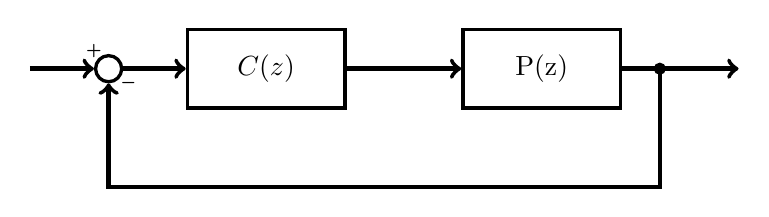
\begin{tikzpicture}[scale=2]
    \node[sum](sum)at(-1,0){};
    \draw[->,ultra thick](-1.5,0)node[above right]{}--(sum.180)node[above]{$\scriptscriptstyle\boldsymbol{+}$};
    \node[block, right of=sum, node distance=2cm](c){$C(z)$};

    \draw[->,ultra thick](sum.0)--(c.180);
  
    \node[block]at(1.75,0)(p){P(z)};
    \draw[->,ultra thick](c.0)--(p.180);

    \filldraw[black](2.5,0)circle(1pt);
    \draw[-,ultra thick](p.0)--(2.5,0);
    \draw[->,ultra thick](2.5,0)--(3,0);
    \draw[->,ultra thick](2.5,0)--(2.5,-0.75)--(-1,-0.75)--(sum.270)node[right]{$\scriptscriptstyle\boldsymbol{-}$};
\end{tikzpicture}
\end{document}